%!TEX root = ../../main.tex
\chapter{Resultate}
Aus den Ergebnissen der vorangegangenen Experimente konnten die optimalen Bedingungen für das Training des Neuronalen Netzes ermittelt werden. Die Standardwerte in Tabelle \ref{table:StandardWerte} sind im Großen und Ganzen gut gewählt, jedoch hat sich aufgrund der Ergebnisse von Experiment 1 in Abschnitt \ref{subsec:1.Experiment} herausgestellt, dass eine geringere Lernrate langfristig einen besseren Erfolg zeigt. Aus diesem Grund wird die Lernrate für das endgültige Modell auf $0.001$ gesetzt. Ebenso wird die Anzahl der Epochen mehr als verdoppelt und auf den Wert 50 gesetzt.

Der Trainingsverlauf, siehe Anhang \ref{appendix:FinalVerlustkurven}, des finalen Modells ist zu Beginn identisch mit dem Modell ''LR0.001`` aus dem ersten Experiment, welches sich als am besten erwiesen hat. Nach 20 Epochen nimmt der Verlust auf dem Trainingsdatensatz bis zum Ende jedoch nur minimal ab. Der Verlauf auf dem Validierungsdatensatz ist ebenfalls identisch mit dem des Modells ``LR0.001'', jedoch konnte durch das längere Training der Verlust weiter auf Werte unter $0.1$ reduziert werden. 

Die Ergebnisse des finalen Modells in Tabelle \ref{table:FinalErgebnisse} zeigen eine deutliche Verbesserung gegenüber dem Standardmodell. Der Dice Koeffizient erreichte Werte von über $92\%$ und der Jaccard Index Werte von über $90\%$. Die Pixel Accuracy hat sich ebenfalls verbessert, ist aber, wie bereits in den vorherigen Abschnitten erwähnt, nicht signifikant. Generell ist eine Verbesserung von ca. $5\%$ durch die geringere Lernrate und das längere Training festzustellen.
\begin{table}[!h]
	\centering
	\begin{tabular}{|c|c|c|c|}
		\hline
		& Dice 				& Jaccard Index 	& Pixel Accuracy \\
		\hline
		\textbf{Final}		& \textbf{92,57} 	& \textbf{90,30}  	& \textbf{99,56}  \\
		\hline
		Standard		& 88,44 			& 85,85  			& 99,22  \\
		\hline
	\end{tabular}
	\caption{Ergebnisse des Finalen Modells (Quelle: Eigene Darstellung)}
	\label{table:FinalErgebnisse}
\end{table}

Die Ergebnisse des Neuronalen Netzes zeigen, dass die Entwicklung durchaus machbar ist und teilweise gute Ergebnisse liefern kann. Die Entwicklung eines Modells ist relativ einfach, sofern bereits ein geeigneter Datensatz vorhanden ist. \\
Dabei ist zu beachten, dass die Vorverarbeitung der Daten für eine gute Performance des Modells unerlässlich ist, wie die Ergebnisse des dritten Experiments in Abschnitt \ref{subsec:3.Experiment} gezeigt haben. Dazu müssen die Daten in eine geeignete Form gebracht werden und sollten möglichst nur relevante Informationen enthalten. Wichtig ist auch eine geeignete Wahl der Hyperparameter, da diese das Training stark beeinflussen. Zudem hängt es auch von den Hyperparametern selbst ab, welche Auswirkungen eine Veränderung mit sich bringt.\\
Das Modell hat immer einen gewissen Verlust, der durch geeignete Methoden weiter reduziert werden kann. Der Verlust macht sich auch bei der Auswertung der Bilder bemerkbar, wo das endgültige Modell in Teilen von der korrekten Segmentierung abweicht, wie Abbildung \ref{fig:segmentation} zeigt.


\begin{figure}
	\centering
	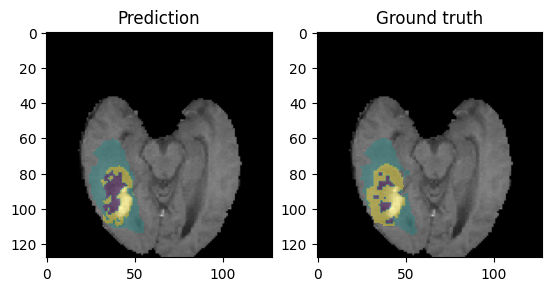
\includegraphics[width=.9\textwidth]{segmentation.png}
	\caption{Links die Segmentierung vom finalen Modell, rechts die wahrhaftige Segmentierung. (Quelle: Eigene Darstellung)}
	\label{fig:segmentation}
\end{figure}